\begin{document}

\chapter{Discussion}
Following \textcite{hamilton2016law}, in which the evaluation is based on examples from previous works on semantic change and words with the ``obsolete'' tag in the Oxford English Dictionary (OED), dictionary entries are consulted to look for ``舊時'' and ``古代'' for attested examples to evaluate the trained diachronic word embeddings.

For example, \zh{齒}{chǐ}{tooth} used to carry the meaning `age (年齡)' and `being of equal rank (並列)' because age determination is made by numbering horses' teeth, which emerges one each year, as in `子之齒長矣,不能事人 (You are long in the tooth)' and `不敢與諸任齒 (I would not dare to take rank equivalent to yours)'; another example is \zh{卑鄙}{bēi-bǐ}{despicable}, which is more neural in connotation in the past \parencite[前言]{wang1997gujinyiyi}. Dictionaries include \textcite{wang1997gujinyiyi,liu1992gujinyi}, which lists word entries with meanings that are distinctive between modern and pre-modern times. Detailed information relavant to semantic change is the number of disyllabic word entries, whether the word convey connotations with varying sentiment polarities, and whether certain senses fall into disuse nowadays, which is valuable resources for the comparison with the results of computational methods. 

The meanings are based on 漢語大字典, 漢語大詞典, 辭源, 辭海 as well as 現代漢語詞典 and 新華詞典 (both published by 商務印書館).

frequency data is derived from 在线古代汉语语料库字频数据\footnote{\url{http://corpus.zhonghuayuwen.org/resources.aspx}} and 近代漢語語料庫詞頻統計\footnote{\url{https://elearning.ling.sinica.edu.tw/jindai.html}}, which are the metadata from the 70-million-word Ancient Chinese Corpus (在线古代汉语语料库) by the Ministry of Education, China and Academia Sinica Tagged Corpus of Early Mandarin Chinese (近代漢語語料庫) by Academia Sinica, Taiwan.

The case study of \jia is based on the assumption that the time-sliced corpus might reflect the similar and different descriptions in language use. While words in \tref{use_case} fall into the categories of technological innovations and ideologies, this study chooses \jia because of its linguistic and cultural characteristics. In pre-modern Chinese, \jia is associated with words that denote physical objects like house.

Because the corpus contains multiple versions of a document, some orthographically-similar characters rank top in terms of cosine similarity scores. However, if compared with the results from \textsc{BOOTSTRAP} samples, the scores are widest. In addition, the ranks vary widely in different iterations, and are a reliable indicator of neighbor analysis. For example, \zh{貧}{pín}{poor;impoverished} appear 43 times out of the 50 iterations as the top 20 closest neighbors, followed by \zh{窶}{jù}{poor;impoverished} also appear 26 times. Other closest neighbors include 族, 世, 妻, 冢, 富, \zh{寠}{jù}{poor;impoverished}, 孀, 糿, 父 (all more than 15 times.)

As for the word 宅, the closest neighbors include 田(48), 廨(47), 居(39), 園(36), 墅(36), 家(35), and 廛(14), filtering out 冢(1). Compared with \textsc{FIXED} embeddings, the closest neighbors for the Tang dynasty include 廨, 田, 宇, 邸, 園, 營, 室, 塋, 寺, 住, 妝, 寓. Therefore, if neighbor analysis can be compared from two directions, it is likely to mitigate the issue arising from OCR errors?

The semantic history of linguistic units or expressions are far more unpredictable than data that contain seasonality. Regarding the closet neighbors for \jia , the results differ in a distinctive way, with a low percentage of overlaps between the \textsc{FIXED} embeddings and the \textsc{BOOTSTRAP} ones. In addition, before the diachronic character-based embeddings are constructed, a decision needs to be made on whether the different versions of a workset of texts are to be included or excluded. Considering the fact that the documents are converted from scanned copies to the digital texts in UTF-8 encoding using the OCR technique, the \textsc{FIXED} embeddings reinforce the parts that are consistently recognizable and transformed into similar strings of characters. In other words, the inclusion of all versions in a workset of documents prevents misrecognized characters from taking up a significant portion of the word occurrence behavior. On the other hand, the word cooccurence profile remains susceptible to orthographically highly similar characters, e.g., 家 and 冢, 人 and 入, and 怡 and 恰, and place the mistaken form as the close neighbors, oftentimes the closest neighbor.

% topic modeling
\begin{figure}[H]
    \centering
    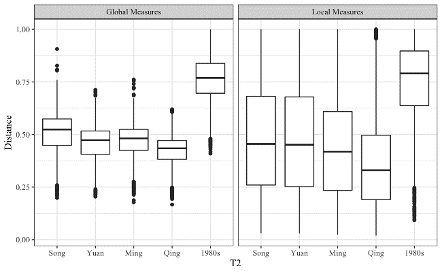
\includegraphics[width=0.95\textwidth,keepaspectratio]{figures/global_local}
    \caption{Distribution of degree of semantic change for global and local measures}
  \end{figure}

Note: Below is the results for semantic change trends based on all of the character-based embeddings, change to example of \jia or group of words only

\cmidnospacing
\begin{table}[H]
    \centering
    \begin{tabular}{c|ccc}
        & w1 & w5 & w10 \\
        \cmidrule{1-4}
        1\sts  order &
        \cincludegraphics[width=0.28\textwidth]{figures/table_VNC/Picture_1-1.png} &
        \cincludegraphics[width=0.28\textwidth]{figures/table_VNC/Picture_1-2.png} &
        \cincludegraphics[width=0.28\textwidth]{figures/table_VNC/Picture_1-3.png} \\
        \makecell{2\nds  order - \\Global measure} &
        \cincludegraphics[width=0.28\textwidth]{figures/table_VNC/Picture_2-1.png} &
        \cincludegraphics[width=0.28\textwidth]{figures/table_VNC/Picture_2-2.png} &
        \cincludegraphics[width=0.28\textwidth]{figures/table_VNC/Picture_2-3.png} \\
        \makecell{2\nds  order - \\Local measure} &
        \cincludegraphics[width=0.28\textwidth]{figures/table_VNC/Picture_3-1.png} &
        \cincludegraphics[width=0.28\textwidth]{figures/table_VNC/Picture_3-2.png} &
        \cincludegraphics[width=0.28\textwidth]{figures/table_VNC/Picture_3-3.png} \\
    \end{tabular}
\end{table}

\end{document}